\section{Workflow from QGIS to CaWaQS Output}

This diagram describes the typical execution flow when a user triggers a computation in the CaWaQS-ViZ QGIS plugin.  
It highlights how the shared \texttt{HydrologicalTwin} instance, created once in \texttt{ExploreData}, propagates through all dialogs and backend services.

\begin{center}
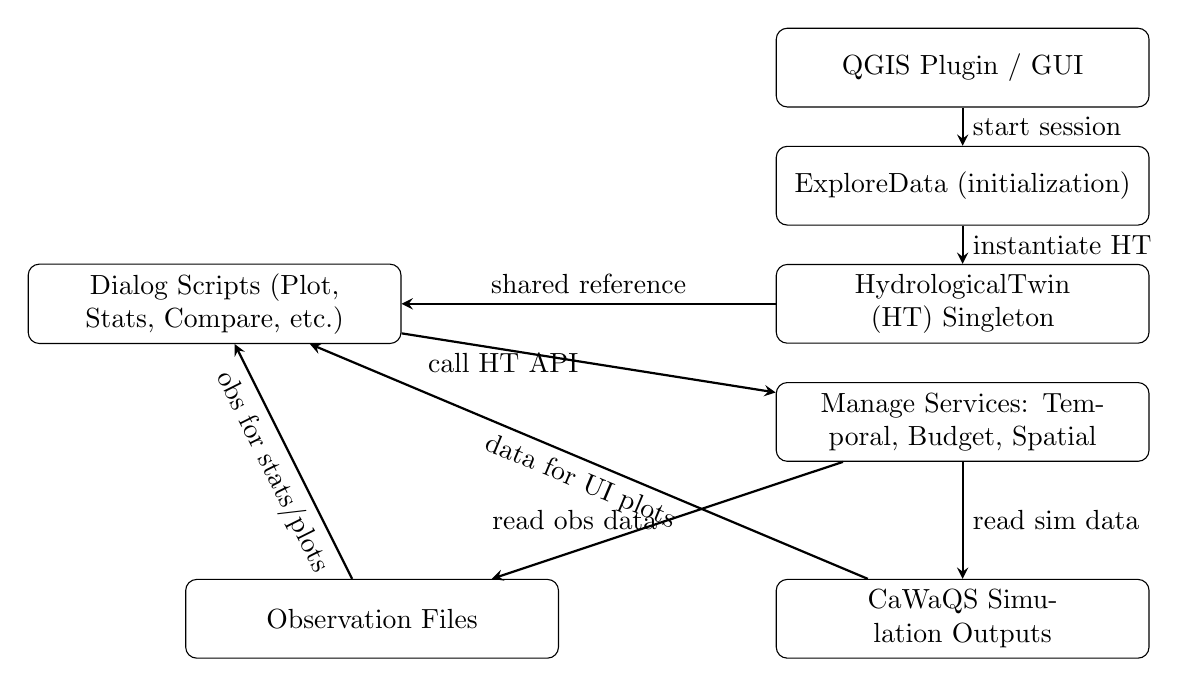
\begin{tikzpicture}[
  node distance=1.5cm,
  box/.style={rectangle, draw, rounded corners, text width=4.5cm, align=center, minimum height=1cm},
  arrow/.style={->, thick, >=stealth}
]

% Nodes
\node[box] (qgis) {QGIS Plugin / GUI};
\node[box, below of=qgis] (explore) {ExploreData (initialization)};
\node[box, below of=explore] (ht) {HydrologicalTwin (HT) Singleton};
\node[box, left of=ht, xshift=-8cm] (dialogs) {Dialog Scripts (Plot, Stats, Compare, etc.)};
\node[box, below of=ht] (services) {Manage Services: Temporal, Budget, Spatial};
\node[box, below of=services, yshift=-1cm] (ca) {CaWaQS Simulation Outputs};
\node[box, left of=ca, xshift=-6cm] (obs) {Observation Files};

% Arrows
\draw[arrow] (qgis) -- (explore) node[midway, right] {start session};
\draw[arrow] (explore) -- (ht) node[midway, right] {instantiate HT};
\draw[arrow] (ht) -- (dialogs) node[midway, above] {shared reference};
\draw[arrow] (dialogs) -- (services) node[midway, left] {call HT API};
\draw[arrow] (services) -- (ca) node[midway, right] {read sim data};
\draw[arrow] (services) -- (obs) node[midway, left] {read obs data};
\draw[arrow] (ca) -- (dialogs) node[midway, below, sloped] {data for UI plots};
\draw[arrow] (obs) -- (dialogs) node[midway, below, sloped] {obs for stats/plots};

\end{tikzpicture}
%\caption{
%        Workflow from QGIS to CaWaQS output.
%        \textbf{Public users} (gray path) are limited to the \textit{Rendering} layer.
%        \textbf{Private-key users} (blue path) access full functionality, with actions %logged for traceability.
%    }

\end{center}
% --- NOUVELLE VERSION DE 3.3.1 ---
\subsection{Description of Workflow Steps}
\label{sec:workflow-steps}

The workflow from QGIS to CaWaQS output is structured to enforce \textbf{access control} and \textbf{reproducibility} at every stage. Figure~\ref{fig:workflow-keys} illustrates the process, with distinct paths for public and private-key users.

\begin{enumerate}

    \item \textbf{QGIS Plugin / UI}
    The user interacts with the QGIS interface and triggers an action (e.g., plot simulation, compare sim/obs, calculate statistics). The plugin initializes the session and checks the user's access level:
    \begin{itemize}
        \item \textbf{Public users} (no private-key) are restricted to visualization and masked data.
        \item \textbf{Private-key users} unlock full functionality, including data extraction and simulation execution.
    \end{itemize}

    \item \textbf{ExploreData Initialization}
    Upon project load, \texttt{ExploreData.get\_instance()} is called, constructing a \texttt{HydrologicalTwin} instance with the project configuration. The twin's mode (\texttt{public} or \texttt{private}) is set based on the presence of a valid private-key:
    \begin{verbatim}
        twin = HydrologicalTwin(mode="private", key="user_key.pem")  # Private access
        twin = HydrologicalTwin(mode="public")                       # Public access
    \end{verbatim}

    \item \textbf{HydrologicalTwin Singleton}
    The \texttt{HydrologicalTwin} instance encapsulates all backend services and domain objects. It acts as a gatekeeper:
    \begin{itemize}
        \item Validates private-keys for restricted operations.
        \item Logs all actions with user-specific metadata.
        \item Enforces consistency across dialogs and simulations.
    \end{itemize}
    The instance is stored in \texttt{ExploreData} and reused by all dialogs.

    \item \textbf{Dialog Scripts}
    When a user activates a dialog (e.g., "Compare Sim/Obs"), the dialog retrieves the shared \texttt{HydrologicalTwin} instance and checks permissions:
    \begin{verbatim}
        self.hydro_twin = self.exd.hydro_twin
        if dialog.requires_private_access and not self.hydro_twin.has_key():
            raise PermissionError("Private-key required for this operation.")
    \end{verbatim}
    Dialogs call only \texttt{HydrologicalTwin} API methods (e.g., \texttt{extract\_values}, \texttt{apply\_temporal\_operator}).

    \item \textbf{Private-Key Validation}
    For restricted operations (e.g., data extraction, parameter modification), the twin verifies the user's private-key:
    \begin{itemize}
        \item If valid, the operation proceeds, and results are cryptographically logged.
        \item If invalid, the twin raises an error:
        \begin{verbatim}
        Error: Private-key required for this operation.
        \end{verbatim}
    \end{itemize}

    \item \textbf{Manage.* Services}
    The twin delegates tasks to internal services (\texttt{Manage.Temporal}, \texttt{Manage.Budget}, \texttt{Manage.Spatial}) with access control:
    \begin{itemize}
        \item \textbf{Public operations} (e.g., rendering maps):
        \begin{verbatim}
            data = twin.apply_spatial_mask(request)  # Masked/aggregated data
        \end{verbatim}
        \item \textbf{Private operations} (e.g., raw data extraction):
        \begin{verbatim}
            data = twin.extract_values(request)      # Requires private-key
        \end{verbatim}
    \end{itemize}
    Services perform:
    \begin{itemize}
        \item Temporal/spatial aggregation (e.g., annual mean, catchment-level averages).
        \item Budget calculations and statistical analyses.
        \item GIS-based spatial operations (e.g., catchment cell extraction).
    \end{itemize}

    \item \textbf{CaWaQS Simulation Output Files}
    Backend services read CaWaQS binary outputs (\texttt{*.bin}) and convert them to NumPy hypercubes. Private-key users access full-resolution data; public users receive masked subsets.

    \item \textbf{Observation Files}
    Observed time series (\texttt{*.dat}) are aligned with simulation periods. Access is restricted based on user permissions:
    \begin{itemize}
        \item Public: Pre-computed statistics or aggregated time series.
        \item Private: Raw observational data.
    \end{itemize}

    \item \textbf{Metadata Verification}
    Before returning results, the twin verifies:
    \begin{itemize}
        \item Consistency of \texttt{GitSynchroRecord} hashes for code, data, and parameters.
        \item Cryptographic signatures for private actions.
    \end{itemize}
    Inconsistencies trigger:
    \begin{verbatim}
    Error: Metadata mismatch. Data or code may have been altered.
    \end{verbatim}

    \item \textbf{Back to Dialog}
    The dialog receives processed data and updates the UI:
    \begin{itemize}
        \item Plots, tables, or PDF/HTML exports for public users.
        \item Raw data, advanced statistics, or simulation controls for private-key users.
    \end{itemize}
    All private actions are logged with the user's key fingerprint.

\end{enumerate}


% --- FIN DE LA SECTION ---
